\section{Задание 3: Решить линейные уравнения}
    \subsection{Постановка задачи}
        На основе представленной ниже системы дифференциальных уравнений построить генератор псевдо-случайных чисел в диапазоне \( [0, 1] \) с помощью метода Эйлера:
        \[ \dot{x} = \sigma \cdot (y - x); \quad \dot{y} = x \cdot (r - z) - y; \quad \dot{z} = x \cdot y - b \cdot z. \]
        В качестве параметров зерна выбрать следующие: \( x_0, ~ y_0, ~ z_0, ~ dt \) и \( n \). Здесь:
        \[ \begin{aligned}
            &x_0 \in (2.8915, 3.2027), ~
            y_0 \in (1.4296, 1.7365), ~
            z_0 \in (15.2113, 16.1852), \\
            &dt \in (0, 0.1], ~
            n > 100, ~
            \sigma = 10, ~
            r = 28, ~
            b = 2.66;
        \end{aligned} \]
        В качестве источника энтропии использовать \textit{Unix}-время, в качестве итератора использовать параметр \( n \). Генератор чисел основывается на методе Эйлера, в качестве результата выдавать десятичную часть числа \( x_k \) из метода. На каждой итерации метода, \( x_k, y_k \) и \( z_k \) округлять до \textbf{тысяч}, чтобы избежать переполнения. Протестировать и представить графики соотношений значений с точностью до десятых и сотых относительно их количества. Приложить код, и примеры работы. 

    
    \subsection{Решение}
        \begin{figure}[H]
            \centering
            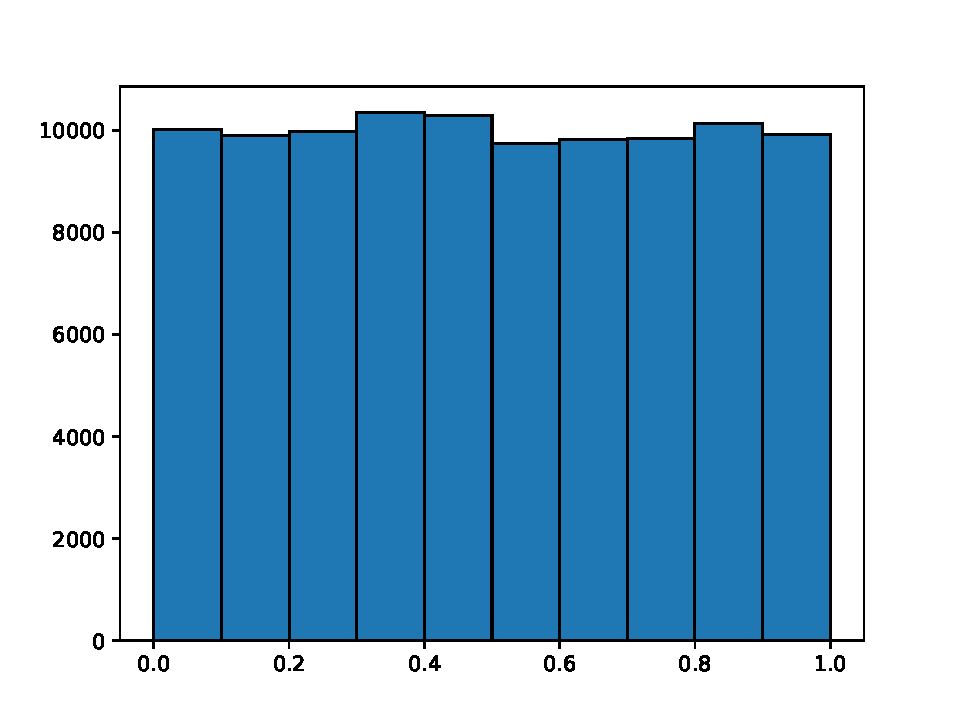
\includegraphics[width=14cm]{pictures/task3_1.pdf}
            \caption{Соотношение значений с точностью до десятых при выборке в 100000.}
        \end{figure}

        \begin{figure}[H]
            \centering
            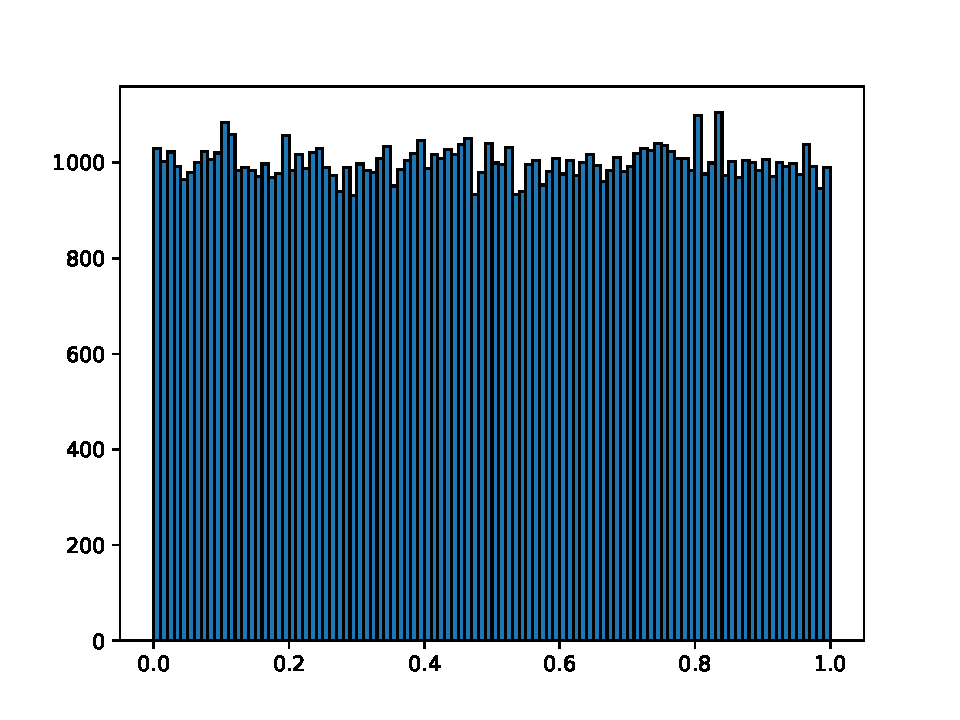
\includegraphics[width=14cm]{pictures/task3_2.pdf}
            \caption{Соотношение значений с точностью до сотых при выборке в 100000.}
        \end{figure}
        
        \lstinputlisting[language=Python,
        caption=Код генератора псевдослучайных чисел,
        style=colored,
        basicstyle=\footnotesize\dejavu,
        frame=lines]{source/task3.py}